% ================================================================
% The printable version of latex/starters/targeted/KS3/percentages/introducingPercentagesStarters.tex
%
% This is the same deck, laid out to be handed out rather than put on
% the board. Every slide is shown as it stands before any answer is
% revealed, and 4 copies of it go on one page of A4, two by two, so
% that a printed page cuts into four question sheets.
%
% Every slide of the deck is here, the title page included, and each takes
% exactly one page. So page 1 is the first slide, page 2 the second, and
% printing the pages you want is how you print the starters you want.
%
%   made from           latex/starters/targeted/KS3/percentages/introducingPercentagesStarters.tex
%   pages on the sheet  6, one per slide of the deck
%   copies of each      4, two by two on A4 landscape
%   printing rules      version 3
%
% Nothing was reworded, nothing was rewritten and nothing was left out.
% Each slide is the slide from the deck, asked for at its first step,
% which is how the answers stay hidden.
%
% Please don't edit this file. It is written again from the one it was
% made from whenever that changes, so an edit here would be lost - edit
% that file instead and this one follows.
% ================================================================
\documentclass{beamer}
\usepackage{tikz}
\usetikzlibrary{calc}
\usepackage{xcolor}
\usepackage{multicol}
\usepackage{amsmath}

% ================================================================
% Answer-overlay helpers
% ================================================================
\newcommand{\ablank}[1]{%
  \alt<2>{\textcolor{red}{#1}}{\underline{\phantom{#1}}}%
}
\newcommand{\ashow}[1]{\uncover<2->{\textcolor{red}{\small #1}}}
\newcommand{\ashowq}[1]{\alt<2->{\textcolor{red}{\small #1}}{?}}

% Answers drawn straight on to a TikZ diagram, revealed on overlay 2 like \ashow.
% Space is reserved on overlay 1, so the diagram does not move between slides.
\usetikzlibrary{overlay-beamer-styles}
\tikzset{
  ans/.style     = {red, thick, visible on=<2->},
  ansfill/.style = {red!15, visible on=<2->},
  anslab/.style  = {red, font=\tiny, visible on=<2->},
}

\title{Percentages: Starters}
\author{}
\date{}

% ---------------------------------------------------------------
% Added so this deck prints four slides to a page. Nothing above
% this line was changed.
% ---------------------------------------------------------------
\usepackage{pgfpages}

% 4 slides to a sheet of A4, two by two, with a thin line round each
% so that the page can be cut up.
%
% Each slide keeps a margin of 1mm around it and no more, so the four fill
% the sheet and the pieces they cut into are as big as the paper allows. Only
% one direction actually comes out that tight: a slide is a different shape
% from a quarter of a sheet of A4, so it is scaled to fit and the slack it
% cannot use is left along whichever pair of edges it did not fill.
\pgfpagesuselayout{4 on 1}[a4paper,landscape,border shrink=1mm]
\pgfpageslogicalpageoptions{1}{border code=\pgfusepath{stroke}}
\pgfpageslogicalpageoptions{2}{border code=\pgfusepath{stroke}}
\pgfpageslogicalpageoptions{3}{border code=\pgfusepath{stroke}}
\pgfpageslogicalpageoptions{4}{border code=\pgfusepath{stroke}}

% There is nothing on paper to click, and a slide announcing a new section
% would sit between two copies of the same question and put every page after
% it out of step with the grid.
\setbeamertemplate{navigation symbols}{}
\AtBeginPart{}
\AtBeginSection{}
\AtBeginSubsection{}
\AtBeginSubsubsection{}
\begin{document}

\frame<1>{\titlepage}
\frame<1>{\titlepage}
\frame<1>{\titlepage}
\frame<1>{\titlepage}

%------------------------------------------------------------------
% SLIDE 1: What is a Percentage?
%------------------------------------------------------------------
\begin{frame}<1>[t]{Starter}
\begin{columns}
\column{0.4\textwidth}
\begin{center}
\vspace{-1.5em}
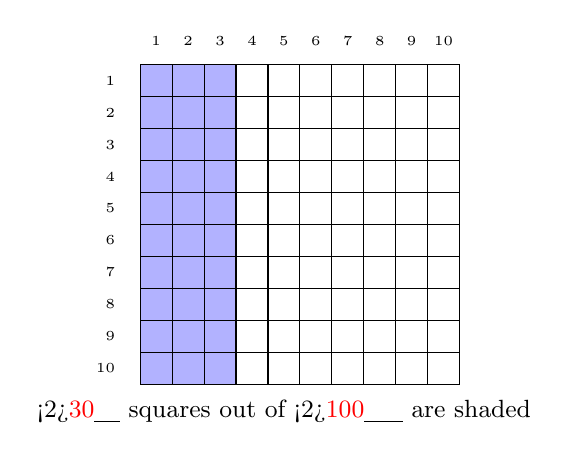
\begin{tikzpicture}[scale=0.78]
% 10×10 grid; first 3 columns shaded = 30 squares
\foreach \col in {0,...,9}{
  \foreach \row in {0,...,9}{
    \ifnum\col<3
      \fill[blue!30] (\col*0.52,\row*0.52) rectangle ++(0.52,0.52);
    \fi
    \draw (\col*0.52,\row*0.52) rectangle ++(0.52,0.52);
  }
}
% Column numbers 1--10 along the top
\foreach \col in {0,...,9}{
  \node[font=\tiny, above] at (\col*0.52+0.26, 5.2+0.15) {\number\numexpr\col+1};
}
% Row numbers 1--10 along the left side (bottom = 1, top = 10)
\foreach \row in {0,...,9}{
  \node[font=\tiny, left] at (-0.25, \row*0.52+0.26) {\number\numexpr10-\row};
}
\node at (2.34,-0.45) {\small \ablank{30} squares out of \ablank{100} are shaded };
\end{tikzpicture}
\end{center}

\column{0.6\textwidth}
\vspace{-1.5em}
\begin{enumerate}
  \item In the diagram how many squares are shaded?
        \ablank{30}
  \item How many total squares are there?
        \ablank{100}
  \item $70 + 30 = \ablank{100}$
  \item $25 \times 4 = \ablank{100}$
  \item What fraction of the square is shaded:
        \ashow{$\tfrac{30}{100}$}
  \item ``Per cent'' means ``out of \ablank{100}''.
  \item The shaded fraction $= \ablank{30\%}$
  \item Write $\dfrac{1}{2}$ as a percentage. \ablank{$50\%$}
  \item Write $\dfrac{1}{4}$ as a percentage. \ablank{$25\%$}
  \item Write $\dfrac{5}{4}$ as a percentage. \ablank{$125\%$}
\end{enumerate}
\end{columns}
\end{frame}
\begin{frame}<1>[t]{Starter}
\begin{columns}
\column{0.4\textwidth}
\begin{center}
\vspace{-1.5em}
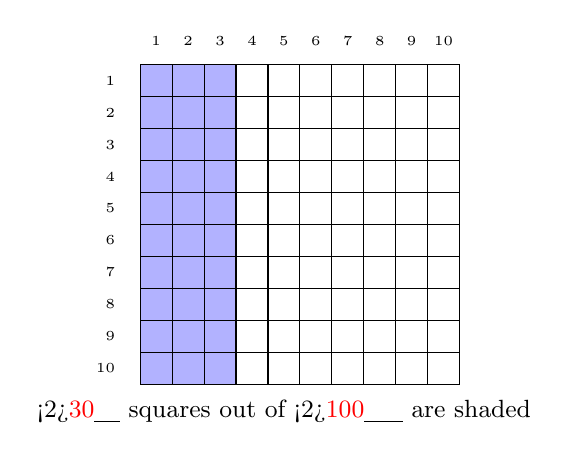
\begin{tikzpicture}[scale=0.78]
% 10×10 grid; first 3 columns shaded = 30 squares
\foreach \col in {0,...,9}{
  \foreach \row in {0,...,9}{
    \ifnum\col<3
      \fill[blue!30] (\col*0.52,\row*0.52) rectangle ++(0.52,0.52);
    \fi
    \draw (\col*0.52,\row*0.52) rectangle ++(0.52,0.52);
  }
}
% Column numbers 1--10 along the top
\foreach \col in {0,...,9}{
  \node[font=\tiny, above] at (\col*0.52+0.26, 5.2+0.15) {\number\numexpr\col+1};
}
% Row numbers 1--10 along the left side (bottom = 1, top = 10)
\foreach \row in {0,...,9}{
  \node[font=\tiny, left] at (-0.25, \row*0.52+0.26) {\number\numexpr10-\row};
}
\node at (2.34,-0.45) {\small \ablank{30} squares out of \ablank{100} are shaded };
\end{tikzpicture}
\end{center}

\column{0.6\textwidth}
\vspace{-1.5em}
\begin{enumerate}
  \item In the diagram how many squares are shaded?
        \ablank{30}
  \item How many total squares are there?
        \ablank{100}
  \item $70 + 30 = \ablank{100}$
  \item $25 \times 4 = \ablank{100}$
  \item What fraction of the square is shaded:
        \ashow{$\tfrac{30}{100}$}
  \item ``Per cent'' means ``out of \ablank{100}''.
  \item The shaded fraction $= \ablank{30\%}$
  \item Write $\dfrac{1}{2}$ as a percentage. \ablank{$50\%$}
  \item Write $\dfrac{1}{4}$ as a percentage. \ablank{$25\%$}
  \item Write $\dfrac{5}{4}$ as a percentage. \ablank{$125\%$}
\end{enumerate}
\end{columns}
\end{frame}
\begin{frame}<1>[t]{Starter}
\begin{columns}
\column{0.4\textwidth}
\begin{center}
\vspace{-1.5em}
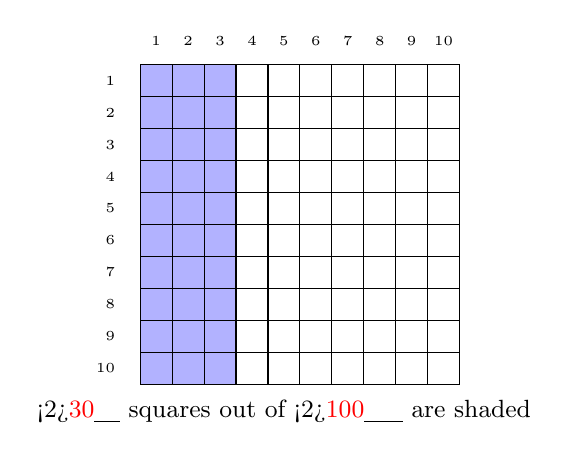
\begin{tikzpicture}[scale=0.78]
% 10×10 grid; first 3 columns shaded = 30 squares
\foreach \col in {0,...,9}{
  \foreach \row in {0,...,9}{
    \ifnum\col<3
      \fill[blue!30] (\col*0.52,\row*0.52) rectangle ++(0.52,0.52);
    \fi
    \draw (\col*0.52,\row*0.52) rectangle ++(0.52,0.52);
  }
}
% Column numbers 1--10 along the top
\foreach \col in {0,...,9}{
  \node[font=\tiny, above] at (\col*0.52+0.26, 5.2+0.15) {\number\numexpr\col+1};
}
% Row numbers 1--10 along the left side (bottom = 1, top = 10)
\foreach \row in {0,...,9}{
  \node[font=\tiny, left] at (-0.25, \row*0.52+0.26) {\number\numexpr10-\row};
}
\node at (2.34,-0.45) {\small \ablank{30} squares out of \ablank{100} are shaded };
\end{tikzpicture}
\end{center}

\column{0.6\textwidth}
\vspace{-1.5em}
\begin{enumerate}
  \item In the diagram how many squares are shaded?
        \ablank{30}
  \item How many total squares are there?
        \ablank{100}
  \item $70 + 30 = \ablank{100}$
  \item $25 \times 4 = \ablank{100}$
  \item What fraction of the square is shaded:
        \ashow{$\tfrac{30}{100}$}
  \item ``Per cent'' means ``out of \ablank{100}''.
  \item The shaded fraction $= \ablank{30\%}$
  \item Write $\dfrac{1}{2}$ as a percentage. \ablank{$50\%$}
  \item Write $\dfrac{1}{4}$ as a percentage. \ablank{$25\%$}
  \item Write $\dfrac{5}{4}$ as a percentage. \ablank{$125\%$}
\end{enumerate}
\end{columns}
\end{frame}
\begin{frame}<1>[t]{Starter}
\begin{columns}
\column{0.4\textwidth}
\begin{center}
\vspace{-1.5em}
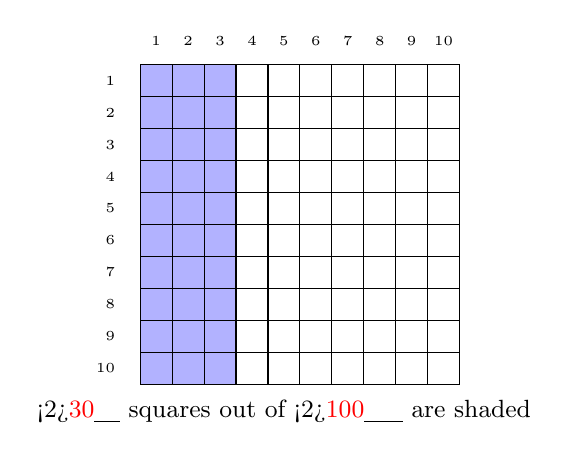
\begin{tikzpicture}[scale=0.78]
% 10×10 grid; first 3 columns shaded = 30 squares
\foreach \col in {0,...,9}{
  \foreach \row in {0,...,9}{
    \ifnum\col<3
      \fill[blue!30] (\col*0.52,\row*0.52) rectangle ++(0.52,0.52);
    \fi
    \draw (\col*0.52,\row*0.52) rectangle ++(0.52,0.52);
  }
}
% Column numbers 1--10 along the top
\foreach \col in {0,...,9}{
  \node[font=\tiny, above] at (\col*0.52+0.26, 5.2+0.15) {\number\numexpr\col+1};
}
% Row numbers 1--10 along the left side (bottom = 1, top = 10)
\foreach \row in {0,...,9}{
  \node[font=\tiny, left] at (-0.25, \row*0.52+0.26) {\number\numexpr10-\row};
}
\node at (2.34,-0.45) {\small \ablank{30} squares out of \ablank{100} are shaded };
\end{tikzpicture}
\end{center}

\column{0.6\textwidth}
\vspace{-1.5em}
\begin{enumerate}
  \item In the diagram how many squares are shaded?
        \ablank{30}
  \item How many total squares are there?
        \ablank{100}
  \item $70 + 30 = \ablank{100}$
  \item $25 \times 4 = \ablank{100}$
  \item What fraction of the square is shaded:
        \ashow{$\tfrac{30}{100}$}
  \item ``Per cent'' means ``out of \ablank{100}''.
  \item The shaded fraction $= \ablank{30\%}$
  \item Write $\dfrac{1}{2}$ as a percentage. \ablank{$50\%$}
  \item Write $\dfrac{1}{4}$ as a percentage. \ablank{$25\%$}
  \item Write $\dfrac{5}{4}$ as a percentage. \ablank{$125\%$}
\end{enumerate}
\end{columns}
\end{frame}

%------------------------------------------------------------------
% SLIDE 2: Fractions → Percentages (denominator divides 100)
%------------------------------------------------------------------
\begin{frame}<1>[t]{Starter}
\begin{columns}
\column{0.48\textwidth}
\vspace{-4em}
\begin{center}
% \vspace{-1.5em}
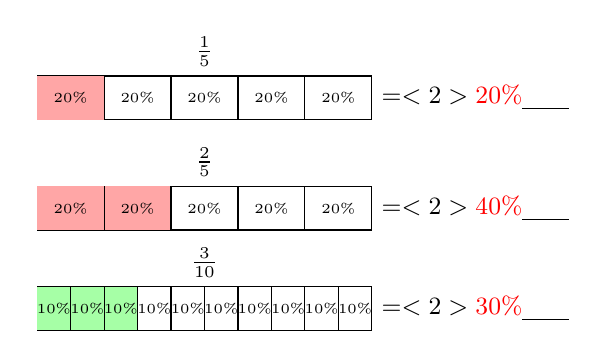
\begin{tikzpicture}[scale=0.85]
% bar 1/5
\draw (0,0) rectangle (5.0,0.65);
\fill[red!35] (0,0) rectangle (1.0,0.65);
\foreach \x in {1,2,3,4} \draw (\x,0) -- (\x,0.65);
\foreach \i in {0,1,2,3,4}
  \node[font=\tiny] at (\i +0.50,0.325) {20\%};
\node[above,font=\small] at (2.5,0.65) {$\tfrac{1}{5}$};
\node[right,font=\small] at (5.0,0.325) {$=\ablank{20\%}$};

% bar 2/5
\draw (0,-1.65) rectangle (5.0,-1.0);
\fill[red!35] (0,-1.65) rectangle (2.0,-1.0);
\foreach \x in {1,2,3,4} \draw (\x,-1.65) -- (\x,-1.0);
\foreach \i in {0,1,2,3,4}
  \node[font=\tiny] at (\i+0.50,-1.325) {20\%};
\node[above,font=\small] at (2.5,-1.0) {$\tfrac{2}{5}$};
\node[right,font=\small] at (5.0,-1.325) {$=\ablank{40\%}$};

% bar 3/10 (lowered further for extra separation)
\draw (0,-3.15) rectangle (5.0,-2.5);
\fill[green!35] (0,-3.15) rectangle (1.50,-2.5);
\foreach \x in {0.50,1.0,...,5.00} \draw (\x,-3.15) -- (\x,-2.5);
\foreach \i in {0,...,9}
  \node[font=\tiny] at (\i*0.50+0.25,-2.825) {10\%};
\node[above,font=\small] at (2.5,-2.5) {$\tfrac{3}{10}$};
\node[right,font=\small] at (5.0,-2.825) {$=\ablank{30\%}$};
\end{tikzpicture}
\end{center}

\column{0.52\textwidth}

\vspace{-2em}
\begin{multicols}{2}
\begin{enumerate}
   \setlength{\itemsep}{12pt}
  \item $3 \times 20 = \ablank{60}$
  \item $7 \times 10 = \ablank{70}$
  \item $\dfrac{1}{5} = \ablank{20\%}$
  \item $\dfrac{2}{5} = \ablank{40\%}$
  \item $\dfrac{3}{10} = \ablank{30\%}$
  \item $\dfrac{\text{\ashowq{7}}}{10} = 70\%$
  \item $\dfrac{1}{\text{\ashowq{4}}} = 25\%$
  \item $\dfrac{2}{25} = \ablank{8\%}$
  \item $\dfrac{7}{8} = \ablank{87.5\%}$
  \end{enumerate}
\end{multicols}
\begin{center}
  \begin{enumerate}
  \setcounter{enumi}{9}
  \item $\dfrac{5}{3}={}$\ablank{$166.\dot{6}\%$}
  \vspace{0.6em}
  \item Complete the conversion: \\[2pt]
        $\dfrac{\text{\ashowq{3}}}{4} = \dfrac{75}{\text{\ashowq{100}}} = 75\%$
\end{enumerate}
\end{center}


\end{columns}
\end{frame}
\begin{frame}<1>[t]{Starter}
\begin{columns}
\column{0.48\textwidth}
\vspace{-4em}
\begin{center}
% \vspace{-1.5em}
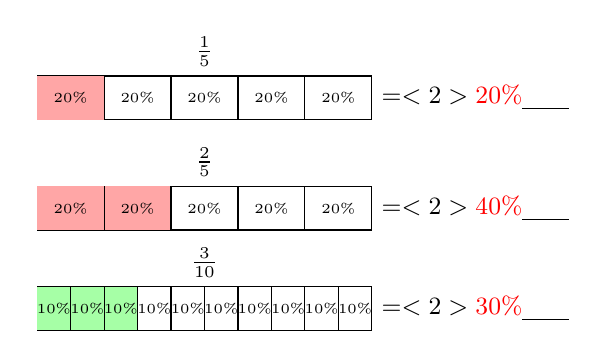
\begin{tikzpicture}[scale=0.85]
% bar 1/5
\draw (0,0) rectangle (5.0,0.65);
\fill[red!35] (0,0) rectangle (1.0,0.65);
\foreach \x in {1,2,3,4} \draw (\x,0) -- (\x,0.65);
\foreach \i in {0,1,2,3,4}
  \node[font=\tiny] at (\i +0.50,0.325) {20\%};
\node[above,font=\small] at (2.5,0.65) {$\tfrac{1}{5}$};
\node[right,font=\small] at (5.0,0.325) {$=\ablank{20\%}$};

% bar 2/5
\draw (0,-1.65) rectangle (5.0,-1.0);
\fill[red!35] (0,-1.65) rectangle (2.0,-1.0);
\foreach \x in {1,2,3,4} \draw (\x,-1.65) -- (\x,-1.0);
\foreach \i in {0,1,2,3,4}
  \node[font=\tiny] at (\i+0.50,-1.325) {20\%};
\node[above,font=\small] at (2.5,-1.0) {$\tfrac{2}{5}$};
\node[right,font=\small] at (5.0,-1.325) {$=\ablank{40\%}$};

% bar 3/10 (lowered further for extra separation)
\draw (0,-3.15) rectangle (5.0,-2.5);
\fill[green!35] (0,-3.15) rectangle (1.50,-2.5);
\foreach \x in {0.50,1.0,...,5.00} \draw (\x,-3.15) -- (\x,-2.5);
\foreach \i in {0,...,9}
  \node[font=\tiny] at (\i*0.50+0.25,-2.825) {10\%};
\node[above,font=\small] at (2.5,-2.5) {$\tfrac{3}{10}$};
\node[right,font=\small] at (5.0,-2.825) {$=\ablank{30\%}$};
\end{tikzpicture}
\end{center}

\column{0.52\textwidth}

\vspace{-2em}
\begin{multicols}{2}
\begin{enumerate}
   \setlength{\itemsep}{12pt}
  \item $3 \times 20 = \ablank{60}$
  \item $7 \times 10 = \ablank{70}$
  \item $\dfrac{1}{5} = \ablank{20\%}$
  \item $\dfrac{2}{5} = \ablank{40\%}$
  \item $\dfrac{3}{10} = \ablank{30\%}$
  \item $\dfrac{\text{\ashowq{7}}}{10} = 70\%$
  \item $\dfrac{1}{\text{\ashowq{4}}} = 25\%$
  \item $\dfrac{2}{25} = \ablank{8\%}$
  \item $\dfrac{7}{8} = \ablank{87.5\%}$
  \end{enumerate}
\end{multicols}
\begin{center}
  \begin{enumerate}
  \setcounter{enumi}{9}
  \item $\dfrac{5}{3}={}$\ablank{$166.\dot{6}\%$}
  \vspace{0.6em}
  \item Complete the conversion: \\[2pt]
        $\dfrac{\text{\ashowq{3}}}{4} = \dfrac{75}{\text{\ashowq{100}}} = 75\%$
\end{enumerate}
\end{center}


\end{columns}
\end{frame}
\begin{frame}<1>[t]{Starter}
\begin{columns}
\column{0.48\textwidth}
\vspace{-4em}
\begin{center}
% \vspace{-1.5em}
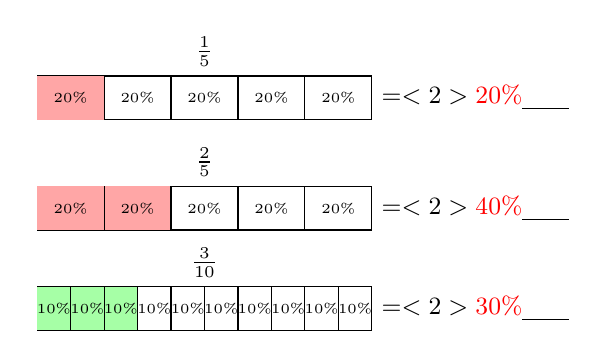
\begin{tikzpicture}[scale=0.85]
% bar 1/5
\draw (0,0) rectangle (5.0,0.65);
\fill[red!35] (0,0) rectangle (1.0,0.65);
\foreach \x in {1,2,3,4} \draw (\x,0) -- (\x,0.65);
\foreach \i in {0,1,2,3,4}
  \node[font=\tiny] at (\i +0.50,0.325) {20\%};
\node[above,font=\small] at (2.5,0.65) {$\tfrac{1}{5}$};
\node[right,font=\small] at (5.0,0.325) {$=\ablank{20\%}$};

% bar 2/5
\draw (0,-1.65) rectangle (5.0,-1.0);
\fill[red!35] (0,-1.65) rectangle (2.0,-1.0);
\foreach \x in {1,2,3,4} \draw (\x,-1.65) -- (\x,-1.0);
\foreach \i in {0,1,2,3,4}
  \node[font=\tiny] at (\i+0.50,-1.325) {20\%};
\node[above,font=\small] at (2.5,-1.0) {$\tfrac{2}{5}$};
\node[right,font=\small] at (5.0,-1.325) {$=\ablank{40\%}$};

% bar 3/10 (lowered further for extra separation)
\draw (0,-3.15) rectangle (5.0,-2.5);
\fill[green!35] (0,-3.15) rectangle (1.50,-2.5);
\foreach \x in {0.50,1.0,...,5.00} \draw (\x,-3.15) -- (\x,-2.5);
\foreach \i in {0,...,9}
  \node[font=\tiny] at (\i*0.50+0.25,-2.825) {10\%};
\node[above,font=\small] at (2.5,-2.5) {$\tfrac{3}{10}$};
\node[right,font=\small] at (5.0,-2.825) {$=\ablank{30\%}$};
\end{tikzpicture}
\end{center}

\column{0.52\textwidth}

\vspace{-2em}
\begin{multicols}{2}
\begin{enumerate}
   \setlength{\itemsep}{12pt}
  \item $3 \times 20 = \ablank{60}$
  \item $7 \times 10 = \ablank{70}$
  \item $\dfrac{1}{5} = \ablank{20\%}$
  \item $\dfrac{2}{5} = \ablank{40\%}$
  \item $\dfrac{3}{10} = \ablank{30\%}$
  \item $\dfrac{\text{\ashowq{7}}}{10} = 70\%$
  \item $\dfrac{1}{\text{\ashowq{4}}} = 25\%$
  \item $\dfrac{2}{25} = \ablank{8\%}$
  \item $\dfrac{7}{8} = \ablank{87.5\%}$
  \end{enumerate}
\end{multicols}
\begin{center}
  \begin{enumerate}
  \setcounter{enumi}{9}
  \item $\dfrac{5}{3}={}$\ablank{$166.\dot{6}\%$}
  \vspace{0.6em}
  \item Complete the conversion: \\[2pt]
        $\dfrac{\text{\ashowq{3}}}{4} = \dfrac{75}{\text{\ashowq{100}}} = 75\%$
\end{enumerate}
\end{center}


\end{columns}
\end{frame}
\begin{frame}<1>[t]{Starter}
\begin{columns}
\column{0.48\textwidth}
\vspace{-4em}
\begin{center}
% \vspace{-1.5em}
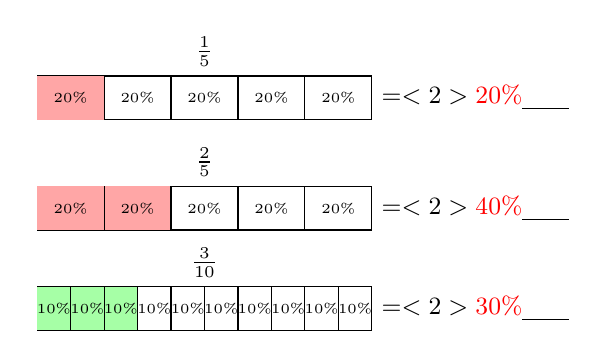
\begin{tikzpicture}[scale=0.85]
% bar 1/5
\draw (0,0) rectangle (5.0,0.65);
\fill[red!35] (0,0) rectangle (1.0,0.65);
\foreach \x in {1,2,3,4} \draw (\x,0) -- (\x,0.65);
\foreach \i in {0,1,2,3,4}
  \node[font=\tiny] at (\i +0.50,0.325) {20\%};
\node[above,font=\small] at (2.5,0.65) {$\tfrac{1}{5}$};
\node[right,font=\small] at (5.0,0.325) {$=\ablank{20\%}$};

% bar 2/5
\draw (0,-1.65) rectangle (5.0,-1.0);
\fill[red!35] (0,-1.65) rectangle (2.0,-1.0);
\foreach \x in {1,2,3,4} \draw (\x,-1.65) -- (\x,-1.0);
\foreach \i in {0,1,2,3,4}
  \node[font=\tiny] at (\i+0.50,-1.325) {20\%};
\node[above,font=\small] at (2.5,-1.0) {$\tfrac{2}{5}$};
\node[right,font=\small] at (5.0,-1.325) {$=\ablank{40\%}$};

% bar 3/10 (lowered further for extra separation)
\draw (0,-3.15) rectangle (5.0,-2.5);
\fill[green!35] (0,-3.15) rectangle (1.50,-2.5);
\foreach \x in {0.50,1.0,...,5.00} \draw (\x,-3.15) -- (\x,-2.5);
\foreach \i in {0,...,9}
  \node[font=\tiny] at (\i*0.50+0.25,-2.825) {10\%};
\node[above,font=\small] at (2.5,-2.5) {$\tfrac{3}{10}$};
\node[right,font=\small] at (5.0,-2.825) {$=\ablank{30\%}$};
\end{tikzpicture}
\end{center}

\column{0.52\textwidth}

\vspace{-2em}
\begin{multicols}{2}
\begin{enumerate}
   \setlength{\itemsep}{12pt}
  \item $3 \times 20 = \ablank{60}$
  \item $7 \times 10 = \ablank{70}$
  \item $\dfrac{1}{5} = \ablank{20\%}$
  \item $\dfrac{2}{5} = \ablank{40\%}$
  \item $\dfrac{3}{10} = \ablank{30\%}$
  \item $\dfrac{\text{\ashowq{7}}}{10} = 70\%$
  \item $\dfrac{1}{\text{\ashowq{4}}} = 25\%$
  \item $\dfrac{2}{25} = \ablank{8\%}$
  \item $\dfrac{7}{8} = \ablank{87.5\%}$
  \end{enumerate}
\end{multicols}
\begin{center}
  \begin{enumerate}
  \setcounter{enumi}{9}
  \item $\dfrac{5}{3}={}$\ablank{$166.\dot{6}\%$}
  \vspace{0.6em}
  \item Complete the conversion: \\[2pt]
        $\dfrac{\text{\ashowq{3}}}{4} = \dfrac{75}{\text{\ashowq{100}}} = 75\%$
\end{enumerate}
\end{center}


\end{columns}
\end{frame}

%------------------------------------------------------------------
% SLIDE 3: Converting Fractions to Percentages (reworked)
%------------------------------------------------------------------
\begin{frame}<1>[t]{Starter}
\begin{columns}
\column{0.35\textwidth}
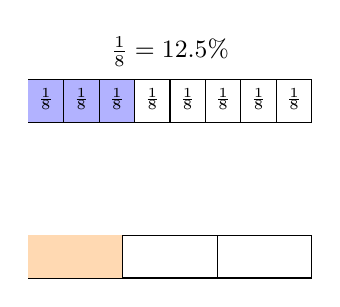
\begin{tikzpicture}[scale=0.9]
% visual bar for 3/8
\draw (0,0) rectangle (4,0.6);
\fill[blue!30] (0,0) rectangle (1.5,0.6);   % 3 of 8 segments
\foreach \x in {0.5,1.0,1.5,2.0,2.5,3.0,3.5}
  \draw (\x,0) -- (\x,0.6);
\foreach \i in {0.5,1.0,1.5,2.0,2.5,3.0,3.5,4.0}
  \node[font=\tiny] at (\i-0.25,0.325) {$\frac{1}{8}$};
  
\node[above,font=\small] at (2,0.65) {$\frac{1}{8} = 12.5\%$};
% second bar for 1/3
\draw (0,-2.2) rectangle (4,-1.6);
\fill[orange!30] (0,-2.2) rectangle (1.333,-1.6);
\draw (1.333,-2.2) -- (1.333,-1.6);
\draw (2.667,-2.2) -- (2.667,-1.6);
\end{tikzpicture}

\column{0.65\textwidth}
\textbf{Questions}
\begin{enumerate}
  \item Write $\frac{1}{2}$ as a percentage. \ablank{$50\%$}
  \item Write $\frac{3}{10}$ as a percentage. \ablank{$30\%$}
  \item What does “per cent” mean? \ablank{out of 100}
  \item Convert $\frac{3}{8}$ to a percentage. \ablank{$37.5\%$}
  \item What percentage of the second bar is shaded orange? \ablank{$33.\dot{3}\%$}
  \item Convert $\frac{2}{3}$ to a percentage. \ablank{$66.\dot{6}\%$}
  \item What is $\frac{4}{3}$ as a percentage, round your percentage to one decimal place. \ablank{$133.3\%$}
  \item What fraction does $0.1\%$ equal? \ashow{$\frac{1}{1000}$}
  \item What fraction does $0.003\%$ equal? \ashow{$\frac{3}{100,000}$}
\end{enumerate}
\end{columns}
\end{frame}
\begin{frame}<1>[t]{Starter}
\begin{columns}
\column{0.35\textwidth}
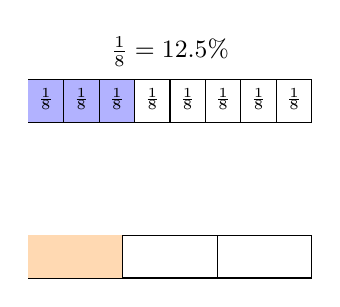
\begin{tikzpicture}[scale=0.9]
% visual bar for 3/8
\draw (0,0) rectangle (4,0.6);
\fill[blue!30] (0,0) rectangle (1.5,0.6);   % 3 of 8 segments
\foreach \x in {0.5,1.0,1.5,2.0,2.5,3.0,3.5}
  \draw (\x,0) -- (\x,0.6);
\foreach \i in {0.5,1.0,1.5,2.0,2.5,3.0,3.5,4.0}
  \node[font=\tiny] at (\i-0.25,0.325) {$\frac{1}{8}$};
  
\node[above,font=\small] at (2,0.65) {$\frac{1}{8} = 12.5\%$};
% second bar for 1/3
\draw (0,-2.2) rectangle (4,-1.6);
\fill[orange!30] (0,-2.2) rectangle (1.333,-1.6);
\draw (1.333,-2.2) -- (1.333,-1.6);
\draw (2.667,-2.2) -- (2.667,-1.6);
\end{tikzpicture}

\column{0.65\textwidth}
\textbf{Questions}
\begin{enumerate}
  \item Write $\frac{1}{2}$ as a percentage. \ablank{$50\%$}
  \item Write $\frac{3}{10}$ as a percentage. \ablank{$30\%$}
  \item What does “per cent” mean? \ablank{out of 100}
  \item Convert $\frac{3}{8}$ to a percentage. \ablank{$37.5\%$}
  \item What percentage of the second bar is shaded orange? \ablank{$33.\dot{3}\%$}
  \item Convert $\frac{2}{3}$ to a percentage. \ablank{$66.\dot{6}\%$}
  \item What is $\frac{4}{3}$ as a percentage, round your percentage to one decimal place. \ablank{$133.3\%$}
  \item What fraction does $0.1\%$ equal? \ashow{$\frac{1}{1000}$}
  \item What fraction does $0.003\%$ equal? \ashow{$\frac{3}{100,000}$}
\end{enumerate}
\end{columns}
\end{frame}
\begin{frame}<1>[t]{Starter}
\begin{columns}
\column{0.35\textwidth}
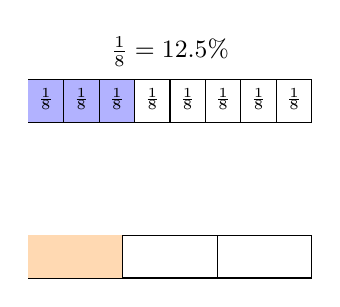
\begin{tikzpicture}[scale=0.9]
% visual bar for 3/8
\draw (0,0) rectangle (4,0.6);
\fill[blue!30] (0,0) rectangle (1.5,0.6);   % 3 of 8 segments
\foreach \x in {0.5,1.0,1.5,2.0,2.5,3.0,3.5}
  \draw (\x,0) -- (\x,0.6);
\foreach \i in {0.5,1.0,1.5,2.0,2.5,3.0,3.5,4.0}
  \node[font=\tiny] at (\i-0.25,0.325) {$\frac{1}{8}$};
  
\node[above,font=\small] at (2,0.65) {$\frac{1}{8} = 12.5\%$};
% second bar for 1/3
\draw (0,-2.2) rectangle (4,-1.6);
\fill[orange!30] (0,-2.2) rectangle (1.333,-1.6);
\draw (1.333,-2.2) -- (1.333,-1.6);
\draw (2.667,-2.2) -- (2.667,-1.6);
\end{tikzpicture}

\column{0.65\textwidth}
\textbf{Questions}
\begin{enumerate}
  \item Write $\frac{1}{2}$ as a percentage. \ablank{$50\%$}
  \item Write $\frac{3}{10}$ as a percentage. \ablank{$30\%$}
  \item What does “per cent” mean? \ablank{out of 100}
  \item Convert $\frac{3}{8}$ to a percentage. \ablank{$37.5\%$}
  \item What percentage of the second bar is shaded orange? \ablank{$33.\dot{3}\%$}
  \item Convert $\frac{2}{3}$ to a percentage. \ablank{$66.\dot{6}\%$}
  \item What is $\frac{4}{3}$ as a percentage, round your percentage to one decimal place. \ablank{$133.3\%$}
  \item What fraction does $0.1\%$ equal? \ashow{$\frac{1}{1000}$}
  \item What fraction does $0.003\%$ equal? \ashow{$\frac{3}{100,000}$}
\end{enumerate}
\end{columns}
\end{frame}
\begin{frame}<1>[t]{Starter}
\begin{columns}
\column{0.35\textwidth}
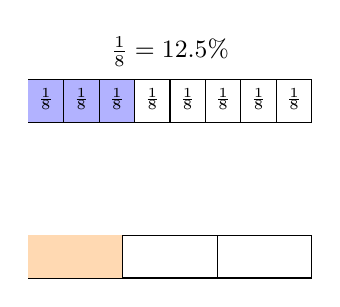
\begin{tikzpicture}[scale=0.9]
% visual bar for 3/8
\draw (0,0) rectangle (4,0.6);
\fill[blue!30] (0,0) rectangle (1.5,0.6);   % 3 of 8 segments
\foreach \x in {0.5,1.0,1.5,2.0,2.5,3.0,3.5}
  \draw (\x,0) -- (\x,0.6);
\foreach \i in {0.5,1.0,1.5,2.0,2.5,3.0,3.5,4.0}
  \node[font=\tiny] at (\i-0.25,0.325) {$\frac{1}{8}$};
  
\node[above,font=\small] at (2,0.65) {$\frac{1}{8} = 12.5\%$};
% second bar for 1/3
\draw (0,-2.2) rectangle (4,-1.6);
\fill[orange!30] (0,-2.2) rectangle (1.333,-1.6);
\draw (1.333,-2.2) -- (1.333,-1.6);
\draw (2.667,-2.2) -- (2.667,-1.6);
\end{tikzpicture}

\column{0.65\textwidth}
\textbf{Questions}
\begin{enumerate}
  \item Write $\frac{1}{2}$ as a percentage. \ablank{$50\%$}
  \item Write $\frac{3}{10}$ as a percentage. \ablank{$30\%$}
  \item What does “per cent” mean? \ablank{out of 100}
  \item Convert $\frac{3}{8}$ to a percentage. \ablank{$37.5\%$}
  \item What percentage of the second bar is shaded orange? \ablank{$33.\dot{3}\%$}
  \item Convert $\frac{2}{3}$ to a percentage. \ablank{$66.\dot{6}\%$}
  \item What is $\frac{4}{3}$ as a percentage, round your percentage to one decimal place. \ablank{$133.3\%$}
  \item What fraction does $0.1\%$ equal? \ashow{$\frac{1}{1000}$}
  \item What fraction does $0.003\%$ equal? \ashow{$\frac{3}{100,000}$}
\end{enumerate}
\end{columns}
\end{frame}

%------------------------------------------------------------------
% SLIDE 4: Adding Fractions and Percentages
%------------------------------------------------------------------
\begin{frame}<1>[t]{Starter}
\begin{columns}
\column{0.35\textwidth}
\begin{center}
\vspace{-5em}
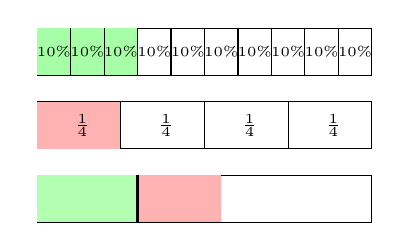
\begin{tikzpicture}[scale=0.85]
% 30% bar
\draw (0,0) rectangle (5.0,0.7);
\fill[green!35] (0,0) rectangle (1.50,0.7);
\foreach \x in {0.50,1.0,...,5.00} \draw (\x,0) -- (\x,0.7);
\foreach \i in {0,...,9}
  \node[font=\tiny] at (\i*0.50+0.25,0.35) {10\%};

% 1/4 = 25% bar
\draw (0,-1.1) rectangle (5,-0.4);
\fill[red!30] (0,-1.1) rectangle (1.25,-0.4);
\foreach \x in {1.25,2.5,3.75} \draw (\x,-1.1) -- (\x,-0.4);
\foreach \i in {0,...,3}
    \node[font=\tiny] at (\i*1.25+0.675,-0.75) {$\frac{1}{4}$};
    
% Combined bar
\draw (0,-2.2) rectangle (5,-1.5);
\fill[green!30] (0,-2.2) rectangle (1.5,-1.5);
\fill[red!30] (1.5,-2.2) rectangle (2.75,-1.5);
\draw[thick] (1.5,-2.2) -- (1.5,-1.5);
\end{tikzpicture}


\end{center}

\column{0.7\textwidth}
\vspace{-2em}
\begin{enumerate}
\begin{multicols}{2}
  \item $50\% + 50\% = \ablank{100\%}$
  \item $25\% + 25\% = \ablank{50\%}$
\end{multicols}
  \item Write $\frac{1}{5}$ as a percentage: \ablank{$20\%$}
  \item Complete the sum represented by the diagram: \\[0.2em]
  $ 3 \times \text{\ashowq{10}}\% + \frac{1}{\text{\ashowq{4}}} = 30\% + 25\% = 55\% $
\begin{multicols}{2}
  \item $20\%+\dfrac{3}{10}=\ablank{50\%}$
  \item $\dfrac{1}{2}+15\%=\ablank{65\%}$
  \item $45\%+\dfrac{1}{5}=\ablank{65\%}$
  \item Which is larger: $\dfrac{3}{8}$ or $40\%$?
        \ablank{$40\%$ ($\tfrac{3}{8}=37.5\%$)}
  \item $\dfrac{2}{5}+\dfrac{3}{10}+20\%=\ablank{90\%}$
\end{multicols}
  
  \item A class finishes $\tfrac{1}{3}$ of a project, then $20\%$ more. What percentage have they completed in total?
        \ashow{$33.\dot{3}\%+20\%=53.\dot{3}\%$}
\end{enumerate}
\end{columns}
\end{frame}
\begin{frame}<1>[t]{Starter}
\begin{columns}
\column{0.35\textwidth}
\begin{center}
\vspace{-5em}
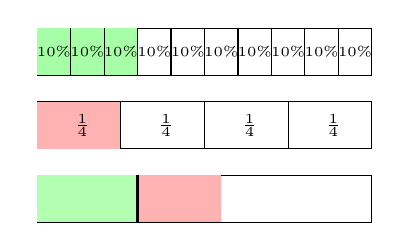
\begin{tikzpicture}[scale=0.85]
% 30% bar
\draw (0,0) rectangle (5.0,0.7);
\fill[green!35] (0,0) rectangle (1.50,0.7);
\foreach \x in {0.50,1.0,...,5.00} \draw (\x,0) -- (\x,0.7);
\foreach \i in {0,...,9}
  \node[font=\tiny] at (\i*0.50+0.25,0.35) {10\%};

% 1/4 = 25% bar
\draw (0,-1.1) rectangle (5,-0.4);
\fill[red!30] (0,-1.1) rectangle (1.25,-0.4);
\foreach \x in {1.25,2.5,3.75} \draw (\x,-1.1) -- (\x,-0.4);
\foreach \i in {0,...,3}
    \node[font=\tiny] at (\i*1.25+0.675,-0.75) {$\frac{1}{4}$};
    
% Combined bar
\draw (0,-2.2) rectangle (5,-1.5);
\fill[green!30] (0,-2.2) rectangle (1.5,-1.5);
\fill[red!30] (1.5,-2.2) rectangle (2.75,-1.5);
\draw[thick] (1.5,-2.2) -- (1.5,-1.5);
\end{tikzpicture}


\end{center}

\column{0.7\textwidth}
\vspace{-2em}
\begin{enumerate}
\begin{multicols}{2}
  \item $50\% + 50\% = \ablank{100\%}$
  \item $25\% + 25\% = \ablank{50\%}$
\end{multicols}
  \item Write $\frac{1}{5}$ as a percentage: \ablank{$20\%$}
  \item Complete the sum represented by the diagram: \\[0.2em]
  $ 3 \times \text{\ashowq{10}}\% + \frac{1}{\text{\ashowq{4}}} = 30\% + 25\% = 55\% $
\begin{multicols}{2}
  \item $20\%+\dfrac{3}{10}=\ablank{50\%}$
  \item $\dfrac{1}{2}+15\%=\ablank{65\%}$
  \item $45\%+\dfrac{1}{5}=\ablank{65\%}$
  \item Which is larger: $\dfrac{3}{8}$ or $40\%$?
        \ablank{$40\%$ ($\tfrac{3}{8}=37.5\%$)}
  \item $\dfrac{2}{5}+\dfrac{3}{10}+20\%=\ablank{90\%}$
\end{multicols}
  
  \item A class finishes $\tfrac{1}{3}$ of a project, then $20\%$ more. What percentage have they completed in total?
        \ashow{$33.\dot{3}\%+20\%=53.\dot{3}\%$}
\end{enumerate}
\end{columns}
\end{frame}
\begin{frame}<1>[t]{Starter}
\begin{columns}
\column{0.35\textwidth}
\begin{center}
\vspace{-5em}
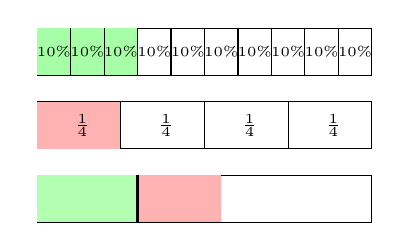
\begin{tikzpicture}[scale=0.85]
% 30% bar
\draw (0,0) rectangle (5.0,0.7);
\fill[green!35] (0,0) rectangle (1.50,0.7);
\foreach \x in {0.50,1.0,...,5.00} \draw (\x,0) -- (\x,0.7);
\foreach \i in {0,...,9}
  \node[font=\tiny] at (\i*0.50+0.25,0.35) {10\%};

% 1/4 = 25% bar
\draw (0,-1.1) rectangle (5,-0.4);
\fill[red!30] (0,-1.1) rectangle (1.25,-0.4);
\foreach \x in {1.25,2.5,3.75} \draw (\x,-1.1) -- (\x,-0.4);
\foreach \i in {0,...,3}
    \node[font=\tiny] at (\i*1.25+0.675,-0.75) {$\frac{1}{4}$};
    
% Combined bar
\draw (0,-2.2) rectangle (5,-1.5);
\fill[green!30] (0,-2.2) rectangle (1.5,-1.5);
\fill[red!30] (1.5,-2.2) rectangle (2.75,-1.5);
\draw[thick] (1.5,-2.2) -- (1.5,-1.5);
\end{tikzpicture}


\end{center}

\column{0.7\textwidth}
\vspace{-2em}
\begin{enumerate}
\begin{multicols}{2}
  \item $50\% + 50\% = \ablank{100\%}$
  \item $25\% + 25\% = \ablank{50\%}$
\end{multicols}
  \item Write $\frac{1}{5}$ as a percentage: \ablank{$20\%$}
  \item Complete the sum represented by the diagram: \\[0.2em]
  $ 3 \times \text{\ashowq{10}}\% + \frac{1}{\text{\ashowq{4}}} = 30\% + 25\% = 55\% $
\begin{multicols}{2}
  \item $20\%+\dfrac{3}{10}=\ablank{50\%}$
  \item $\dfrac{1}{2}+15\%=\ablank{65\%}$
  \item $45\%+\dfrac{1}{5}=\ablank{65\%}$
  \item Which is larger: $\dfrac{3}{8}$ or $40\%$?
        \ablank{$40\%$ ($\tfrac{3}{8}=37.5\%$)}
  \item $\dfrac{2}{5}+\dfrac{3}{10}+20\%=\ablank{90\%}$
\end{multicols}
  
  \item A class finishes $\tfrac{1}{3}$ of a project, then $20\%$ more. What percentage have they completed in total?
        \ashow{$33.\dot{3}\%+20\%=53.\dot{3}\%$}
\end{enumerate}
\end{columns}
\end{frame}
\begin{frame}<1>[t]{Starter}
\begin{columns}
\column{0.35\textwidth}
\begin{center}
\vspace{-5em}
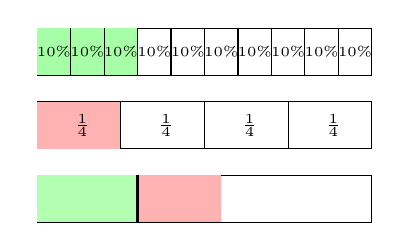
\begin{tikzpicture}[scale=0.85]
% 30% bar
\draw (0,0) rectangle (5.0,0.7);
\fill[green!35] (0,0) rectangle (1.50,0.7);
\foreach \x in {0.50,1.0,...,5.00} \draw (\x,0) -- (\x,0.7);
\foreach \i in {0,...,9}
  \node[font=\tiny] at (\i*0.50+0.25,0.35) {10\%};

% 1/4 = 25% bar
\draw (0,-1.1) rectangle (5,-0.4);
\fill[red!30] (0,-1.1) rectangle (1.25,-0.4);
\foreach \x in {1.25,2.5,3.75} \draw (\x,-1.1) -- (\x,-0.4);
\foreach \i in {0,...,3}
    \node[font=\tiny] at (\i*1.25+0.675,-0.75) {$\frac{1}{4}$};
    
% Combined bar
\draw (0,-2.2) rectangle (5,-1.5);
\fill[green!30] (0,-2.2) rectangle (1.5,-1.5);
\fill[red!30] (1.5,-2.2) rectangle (2.75,-1.5);
\draw[thick] (1.5,-2.2) -- (1.5,-1.5);
\end{tikzpicture}


\end{center}

\column{0.7\textwidth}
\vspace{-2em}
\begin{enumerate}
\begin{multicols}{2}
  \item $50\% + 50\% = \ablank{100\%}$
  \item $25\% + 25\% = \ablank{50\%}$
\end{multicols}
  \item Write $\frac{1}{5}$ as a percentage: \ablank{$20\%$}
  \item Complete the sum represented by the diagram: \\[0.2em]
  $ 3 \times \text{\ashowq{10}}\% + \frac{1}{\text{\ashowq{4}}} = 30\% + 25\% = 55\% $
\begin{multicols}{2}
  \item $20\%+\dfrac{3}{10}=\ablank{50\%}$
  \item $\dfrac{1}{2}+15\%=\ablank{65\%}$
  \item $45\%+\dfrac{1}{5}=\ablank{65\%}$
  \item Which is larger: $\dfrac{3}{8}$ or $40\%$?
        \ablank{$40\%$ ($\tfrac{3}{8}=37.5\%$)}
  \item $\dfrac{2}{5}+\dfrac{3}{10}+20\%=\ablank{90\%}$
\end{multicols}
  
  \item A class finishes $\tfrac{1}{3}$ of a project, then $20\%$ more. What percentage have they completed in total?
        \ashow{$33.\dot{3}\%+20\%=53.\dot{3}\%$}
\end{enumerate}
\end{columns}
\end{frame}

% %------------------------------------------------------------------
% % SLIDE 5: Percentages of Amounts (unchanged)
% %------------------------------------------------------------------
% \begin{frame}[t]{Starter 5: Percentages of Amounts}
% \begin{columns}
% \column{0.40\textwidth}
% \begin{center}
% \begin{tikzpicture}[scale=0.85]
% % 10% of £80
% \draw (0,0) rectangle (3,0.75);
% \foreach \x in {0.3,0.6,...,2.9} \draw (\x,0) -- (\x,0.75);
% \fill[green!35] (0,0) rectangle (0.3,0.75);
% \node[above,font=\small] at (1.5,0.75) {\pounds 80};
% \node[below,font=\tiny] at (0.15,-0.05) {\pounds 8};
% \node[font=\small] at (1.5,-0.42) {$10\%={}$\pounds\ablank{8}};
% % 50% of 60 km
% \draw (0,-1.55) rectangle (3,-0.85);
% \fill[blue!30] (0,-1.55) rectangle (1.5,-0.85);
% \draw (1.5,-1.55) -- (1.5,-0.85);
% \node[above,font=\small] at (1.5,-0.85) {60 km};
% \node[font=\small] at (1.5,-1.95) {$50\%=\ablank{30}$ km};
% % 25% of 200 ml
% \draw (0,-3.0) rectangle (3,-2.35);
% \fill[red!25] (0,-3.0) rectangle (0.75,-2.35);
% \foreach \x in {0.75,1.5,2.25} \draw (\x,-3.0) -- (\x,-2.35);
% \node[above,font=\small] at (1.5,-2.35) {200 ml};
% \node[font=\small] at (1.5,-3.38) {$25\%=\ablank{50}$ ml};
% \end{tikzpicture}
% \end{center}

% \column{0.60\textwidth}
% \textbf{Find the percentage of the amount:}
% \begin{enumerate}
%   \item $10\%$ of \pounds90 $={}$\pounds\ablank{9}
%   \item $50\%$ of \pounds46 $={}$\pounds\ablank{23}
%   \item $25\%$ of $200=\ablank{50}$
%   \item $30\%$ of \pounds50 $={}$\pounds\ablank{15}
%   \item $15\%$ of \pounds80 $={}$\pounds\ablank{12}
%   \item Jacket: \pounds120, reduced by $35\%$. Saving?
%         \ashow{$0.35\times120=\pounds42$}
%   \item $17.5\%$ of \pounds240 $={}$\pounds\ablank{42}
%   \item \textit{Challenge:} 840 pupils; $62.5\%$ go on trip.
%         How many stay?
%         \ashow{$525$ go; $840-525=315$ stay.}
% \end{enumerate}
% \end{columns}
% \end{frame}

% %------------------------------------------------------------------
% % SLIDE 6: Percentage Increase and Decrease (unchanged)
% %------------------------------------------------------------------
% \begin{frame}[t]{Starter 6: Percentage Problems}
% \begin{columns}
% \column{0.40\textwidth}
% \begin{center}
% \begin{tikzpicture}[scale=0.85]
% % Increase arrow
% \draw[thick,->] (0,0.3) -- (3,0.3);
% \node[above,font=\small] at (0,0.3) {\pounds 200};
% \node[above,font=\small] at (3,0.3) {\ablank{\pounds 230}};
% \node[below,font=\small] at (1.5,0.3) {$+15\%$};
% % Decrease arrow
% \draw[thick,->] (0,-0.8) -- (3,-0.8);
% \node[above,font=\small] at (0,-0.8) {80 kg};
% \node[above,font=\small] at (3,-0.8) {\ablank{72 kg}};
% \node[below,font=\small] at (1.5,-0.8) {$-10\%$};
% % Multiplier boxes
% \draw[rounded corners=3pt,thick] (0,-1.9) rectangle (3,-1.3);
% \node[font=\small] at (1.5,-1.6) {$+p\%\ \Rightarrow\ \times\!\left(1+\tfrac{p}{100}\right)$};
% \draw[rounded corners=3pt,thick] (0,-2.85) rectangle (3,-2.1);
% \node[font=\small] at (1.5,-2.48) {$-p\%\ \Rightarrow\ \times\!\left(1-\tfrac{p}{100}\right)$};
% \end{tikzpicture}
% \end{center}

% \column{0.60\textwidth}
% \textbf{Questions}
% \begin{enumerate}
%   \item Increase \pounds60 by $20\%$: \ablank{\pounds72}
%   \item Decrease 150 by $40\%$: \ablank{90}
%   \item Phone: \pounds350, reduced $12\%$. New price?
%         \ashow{$350\times0.88=\pounds308$}
%   \item $60\%$ of 300 students study French.
%         How many? \ablank{180}
%   \item Salary \pounds28\,000 rises $5\%$. New salary?
%         \ashow{$28000\times1.05=\pounds29\,400$}
%   \item VAT at $20\%$ added to \pounds45. Total?
%         \ablank{\pounds54}
%   \item \textit{Challenge:} TV reduced $15\%$ to \pounds340.
%         Original price?
%         \ashow{$340\div0.85=\pounds400$}
% \end{enumerate}
% \end{columns}
% \end{frame}


%------------------------------------------------------------------
% SLIDE 7: Decimals to Percentages
%------------------------------------------------------------------
\begin{frame}<1>[t]{Starter}
\begin{columns}
\column{0.4\textwidth}
\begin{center}
\vspace{-1em}
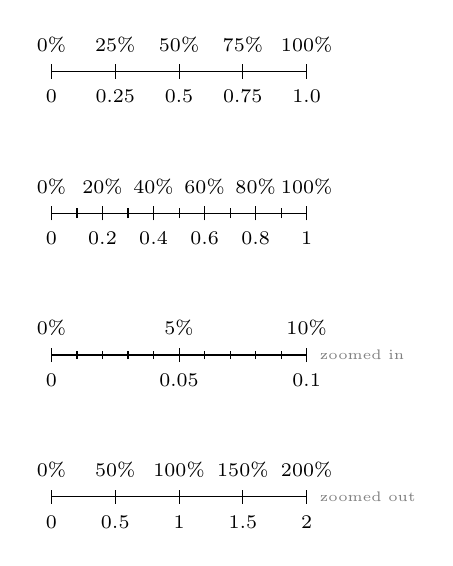
\begin{tikzpicture}[scale=0.9, every node/.style={font=\scriptsize}]

% ── Shared style ──────────────────────────────────────────────
% Each number line: width W, drawn at height Y
% Anchors labelled both sides; target marked with red ? above

% ── LINE 1: 0 to 1 in quarters (scaffolds Q5, Q7, Q3, Q4) ───
\def\Y{0}
\def\W{3.6}
\draw (0,\Y) -- (\W,\Y);
\foreach \frac/\dec/\pct in {%
    0/{0}/{0\%}, 1/{0.25}/{25\%}, 2/{0.5}/{50\%},
    3/{0.75}/{75\%}, 4/{1.0}/{100\%}}{
  \pgfmathsetmacro\xx{\frac*\W/4}
  \draw (\xx,\Y-0.10) -- (\xx,\Y+0.10);
  \node[below] at (\xx,\Y-0.13) {\dec};
  \node[above] at (\xx,\Y+0.13) {\pct};
}
% Target: 0.3 (x = 0.3*W) — red arrow, no answer

% ── LINE 2: 0 to 1 in tenths (scaffolds Q6=0.3, Q12=0.92) ───
\def\Y{-2.0}
\draw (0,\Y) -- (\W,\Y);
\foreach \k in {0,1,...,10}{
  \pgfmathsetmacro\xx{\k*\W/10}
  \pgfmathsetmacro\dec{\k/10}
  \ifodd\k
    \draw (\xx,\Y-0.07) -- (\xx,\Y+0.07); % minor tick
  \else
    \draw (\xx,\Y-0.10) -- (\xx,\Y+0.10);
    \node[below] at (\xx,\Y-0.13) {\pgfmathprintnumber[fixed,precision=1]{\dec}};
    \pgfmathsetmacro\pct{int(\k*10)}
    \node[above] at (\xx,\Y+0.13) {\pct\%};
  \fi
}
% Target: 0.92 — red marker, no answer label
\pgfmathsetmacro\ta{0.92*\W}

% ── LINE 3: 0 to 0.1 zoom (scaffolds Q8=0.08, Q11=0.005) ────
\def\Y{-4.0}
\draw (0,\Y) -- (\W,\Y);
% Anchor ticks at 0, 0.05, 0.1
\foreach \k/\dec/\pct in {0/{0}/{0\%}, 1/{0.05}/{5\%}, 2/{0.1}/{10\%}}{
  \pgfmathsetmacro\xx{\k*\W/2}
  \draw (\xx,\Y-0.10) -- (\xx,\Y+0.10);
  \node[below] at (\xx,\Y-0.13) {\dec};
  \node[above] at (\xx,\Y+0.13) {\pct};
}
% Minor ticks every 0.01
\foreach \k in {1,2,...,9}{
  \pgfmathsetmacro\xx{\k*\W/10}
  \draw (\xx,\Y-0.06) -- (\xx,\Y+0.06);
}
% Target: 0.08
% Zoom label
\node[right,gray] at (\W+0.05,\Y) {\tiny zoomed in};

% ── LINE 4: 0 to 2 (scaffolds Q10=1.4, shows >100%) ─────────
\def\Y{-6.0}
\draw (0,\Y) -- (\W,\Y);
\foreach \k in {0,1,2,3,4}{
  \pgfmathsetmacro\xx{\k*\W/4}
  \pgfmathsetmacro\dec{\k/2}
  \pgfmathsetmacro\pct{int(\k*50)}
  \draw (\xx,\Y-0.10) -- (\xx,\Y+0.10);
  \node[below] at (\xx,\Y-0.13) {\pgfmathprintnumber[fixed,precision=1]{\dec}};
  \node[above] at (\xx,\Y+0.13) {\pct\%};
}

\node[right,gray] at (\W+0.05,\Y) {\tiny zoomed out};

\end{tikzpicture}
\end{center}

\column{0.60\textwidth}
\begin{enumerate}
\begin{multicols}{2}
  \item $0.6 + 0.4 = \ablank{1}$
  \item $0.25 \times 4 = \ablank{1}$
\end{multicols}
  \item Write $\frac{3}{10}$ as a decimal: \ablank{$0.3$}
  \item Write $\frac{7}{100}$ as a decimal: \ablank{$0.07$}
\begin{multicols}{2}
  \item $0.5   = \ablank{50\%}$
  \item $0.3   = \ablank{30\%}$
  \item $0.75  = \ablank{75\%}$
  \item $0.08  = \ablank{8\%}$
  \item $0.125 = \ablank{12.5\%}$
  \item $1.4   = \ablank{140\%}$
  \item $0.005 = \ablank{0.5\%}$
  \item $0.92  \to \ablank{92\%}$
\end{multicols}
  \item \textit{Challenge:} Convert $0.0625$ to a \%,\\
        then write as a fraction in simplest form.
        \ashow{$6.25\%=\tfrac{1}{16}$}
\end{enumerate}
\end{columns}
\end{frame}
\begin{frame}<1>[t]{Starter}
\begin{columns}
\column{0.4\textwidth}
\begin{center}
\vspace{-1em}
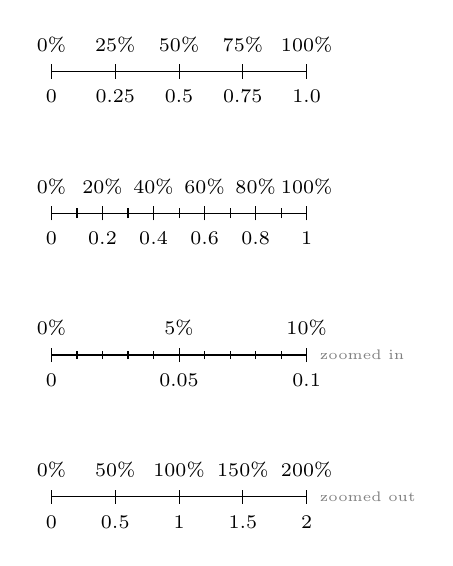
\begin{tikzpicture}[scale=0.9, every node/.style={font=\scriptsize}]

% ── Shared style ──────────────────────────────────────────────
% Each number line: width W, drawn at height Y
% Anchors labelled both sides; target marked with red ? above

% ── LINE 1: 0 to 1 in quarters (scaffolds Q5, Q7, Q3, Q4) ───
\def\Y{0}
\def\W{3.6}
\draw (0,\Y) -- (\W,\Y);
\foreach \frac/\dec/\pct in {%
    0/{0}/{0\%}, 1/{0.25}/{25\%}, 2/{0.5}/{50\%},
    3/{0.75}/{75\%}, 4/{1.0}/{100\%}}{
  \pgfmathsetmacro\xx{\frac*\W/4}
  \draw (\xx,\Y-0.10) -- (\xx,\Y+0.10);
  \node[below] at (\xx,\Y-0.13) {\dec};
  \node[above] at (\xx,\Y+0.13) {\pct};
}
% Target: 0.3 (x = 0.3*W) — red arrow, no answer

% ── LINE 2: 0 to 1 in tenths (scaffolds Q6=0.3, Q12=0.92) ───
\def\Y{-2.0}
\draw (0,\Y) -- (\W,\Y);
\foreach \k in {0,1,...,10}{
  \pgfmathsetmacro\xx{\k*\W/10}
  \pgfmathsetmacro\dec{\k/10}
  \ifodd\k
    \draw (\xx,\Y-0.07) -- (\xx,\Y+0.07); % minor tick
  \else
    \draw (\xx,\Y-0.10) -- (\xx,\Y+0.10);
    \node[below] at (\xx,\Y-0.13) {\pgfmathprintnumber[fixed,precision=1]{\dec}};
    \pgfmathsetmacro\pct{int(\k*10)}
    \node[above] at (\xx,\Y+0.13) {\pct\%};
  \fi
}
% Target: 0.92 — red marker, no answer label
\pgfmathsetmacro\ta{0.92*\W}

% ── LINE 3: 0 to 0.1 zoom (scaffolds Q8=0.08, Q11=0.005) ────
\def\Y{-4.0}
\draw (0,\Y) -- (\W,\Y);
% Anchor ticks at 0, 0.05, 0.1
\foreach \k/\dec/\pct in {0/{0}/{0\%}, 1/{0.05}/{5\%}, 2/{0.1}/{10\%}}{
  \pgfmathsetmacro\xx{\k*\W/2}
  \draw (\xx,\Y-0.10) -- (\xx,\Y+0.10);
  \node[below] at (\xx,\Y-0.13) {\dec};
  \node[above] at (\xx,\Y+0.13) {\pct};
}
% Minor ticks every 0.01
\foreach \k in {1,2,...,9}{
  \pgfmathsetmacro\xx{\k*\W/10}
  \draw (\xx,\Y-0.06) -- (\xx,\Y+0.06);
}
% Target: 0.08
% Zoom label
\node[right,gray] at (\W+0.05,\Y) {\tiny zoomed in};

% ── LINE 4: 0 to 2 (scaffolds Q10=1.4, shows >100%) ─────────
\def\Y{-6.0}
\draw (0,\Y) -- (\W,\Y);
\foreach \k in {0,1,2,3,4}{
  \pgfmathsetmacro\xx{\k*\W/4}
  \pgfmathsetmacro\dec{\k/2}
  \pgfmathsetmacro\pct{int(\k*50)}
  \draw (\xx,\Y-0.10) -- (\xx,\Y+0.10);
  \node[below] at (\xx,\Y-0.13) {\pgfmathprintnumber[fixed,precision=1]{\dec}};
  \node[above] at (\xx,\Y+0.13) {\pct\%};
}

\node[right,gray] at (\W+0.05,\Y) {\tiny zoomed out};

\end{tikzpicture}
\end{center}

\column{0.60\textwidth}
\begin{enumerate}
\begin{multicols}{2}
  \item $0.6 + 0.4 = \ablank{1}$
  \item $0.25 \times 4 = \ablank{1}$
\end{multicols}
  \item Write $\frac{3}{10}$ as a decimal: \ablank{$0.3$}
  \item Write $\frac{7}{100}$ as a decimal: \ablank{$0.07$}
\begin{multicols}{2}
  \item $0.5   = \ablank{50\%}$
  \item $0.3   = \ablank{30\%}$
  \item $0.75  = \ablank{75\%}$
  \item $0.08  = \ablank{8\%}$
  \item $0.125 = \ablank{12.5\%}$
  \item $1.4   = \ablank{140\%}$
  \item $0.005 = \ablank{0.5\%}$
  \item $0.92  \to \ablank{92\%}$
\end{multicols}
  \item \textit{Challenge:} Convert $0.0625$ to a \%,\\
        then write as a fraction in simplest form.
        \ashow{$6.25\%=\tfrac{1}{16}$}
\end{enumerate}
\end{columns}
\end{frame}
\begin{frame}<1>[t]{Starter}
\begin{columns}
\column{0.4\textwidth}
\begin{center}
\vspace{-1em}
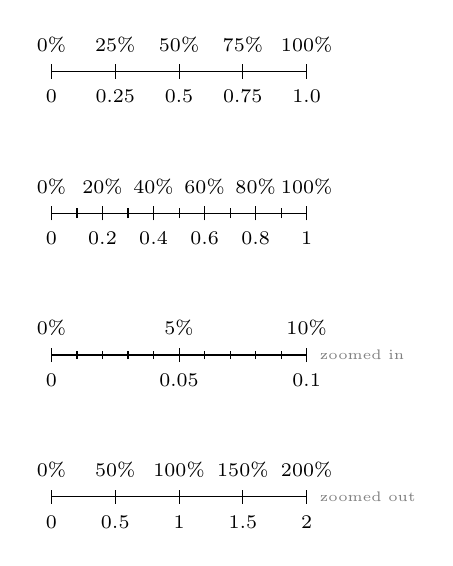
\begin{tikzpicture}[scale=0.9, every node/.style={font=\scriptsize}]

% ── Shared style ──────────────────────────────────────────────
% Each number line: width W, drawn at height Y
% Anchors labelled both sides; target marked with red ? above

% ── LINE 1: 0 to 1 in quarters (scaffolds Q5, Q7, Q3, Q4) ───
\def\Y{0}
\def\W{3.6}
\draw (0,\Y) -- (\W,\Y);
\foreach \frac/\dec/\pct in {%
    0/{0}/{0\%}, 1/{0.25}/{25\%}, 2/{0.5}/{50\%},
    3/{0.75}/{75\%}, 4/{1.0}/{100\%}}{
  \pgfmathsetmacro\xx{\frac*\W/4}
  \draw (\xx,\Y-0.10) -- (\xx,\Y+0.10);
  \node[below] at (\xx,\Y-0.13) {\dec};
  \node[above] at (\xx,\Y+0.13) {\pct};
}
% Target: 0.3 (x = 0.3*W) — red arrow, no answer

% ── LINE 2: 0 to 1 in tenths (scaffolds Q6=0.3, Q12=0.92) ───
\def\Y{-2.0}
\draw (0,\Y) -- (\W,\Y);
\foreach \k in {0,1,...,10}{
  \pgfmathsetmacro\xx{\k*\W/10}
  \pgfmathsetmacro\dec{\k/10}
  \ifodd\k
    \draw (\xx,\Y-0.07) -- (\xx,\Y+0.07); % minor tick
  \else
    \draw (\xx,\Y-0.10) -- (\xx,\Y+0.10);
    \node[below] at (\xx,\Y-0.13) {\pgfmathprintnumber[fixed,precision=1]{\dec}};
    \pgfmathsetmacro\pct{int(\k*10)}
    \node[above] at (\xx,\Y+0.13) {\pct\%};
  \fi
}
% Target: 0.92 — red marker, no answer label
\pgfmathsetmacro\ta{0.92*\W}

% ── LINE 3: 0 to 0.1 zoom (scaffolds Q8=0.08, Q11=0.005) ────
\def\Y{-4.0}
\draw (0,\Y) -- (\W,\Y);
% Anchor ticks at 0, 0.05, 0.1
\foreach \k/\dec/\pct in {0/{0}/{0\%}, 1/{0.05}/{5\%}, 2/{0.1}/{10\%}}{
  \pgfmathsetmacro\xx{\k*\W/2}
  \draw (\xx,\Y-0.10) -- (\xx,\Y+0.10);
  \node[below] at (\xx,\Y-0.13) {\dec};
  \node[above] at (\xx,\Y+0.13) {\pct};
}
% Minor ticks every 0.01
\foreach \k in {1,2,...,9}{
  \pgfmathsetmacro\xx{\k*\W/10}
  \draw (\xx,\Y-0.06) -- (\xx,\Y+0.06);
}
% Target: 0.08
% Zoom label
\node[right,gray] at (\W+0.05,\Y) {\tiny zoomed in};

% ── LINE 4: 0 to 2 (scaffolds Q10=1.4, shows >100%) ─────────
\def\Y{-6.0}
\draw (0,\Y) -- (\W,\Y);
\foreach \k in {0,1,2,3,4}{
  \pgfmathsetmacro\xx{\k*\W/4}
  \pgfmathsetmacro\dec{\k/2}
  \pgfmathsetmacro\pct{int(\k*50)}
  \draw (\xx,\Y-0.10) -- (\xx,\Y+0.10);
  \node[below] at (\xx,\Y-0.13) {\pgfmathprintnumber[fixed,precision=1]{\dec}};
  \node[above] at (\xx,\Y+0.13) {\pct\%};
}

\node[right,gray] at (\W+0.05,\Y) {\tiny zoomed out};

\end{tikzpicture}
\end{center}

\column{0.60\textwidth}
\begin{enumerate}
\begin{multicols}{2}
  \item $0.6 + 0.4 = \ablank{1}$
  \item $0.25 \times 4 = \ablank{1}$
\end{multicols}
  \item Write $\frac{3}{10}$ as a decimal: \ablank{$0.3$}
  \item Write $\frac{7}{100}$ as a decimal: \ablank{$0.07$}
\begin{multicols}{2}
  \item $0.5   = \ablank{50\%}$
  \item $0.3   = \ablank{30\%}$
  \item $0.75  = \ablank{75\%}$
  \item $0.08  = \ablank{8\%}$
  \item $0.125 = \ablank{12.5\%}$
  \item $1.4   = \ablank{140\%}$
  \item $0.005 = \ablank{0.5\%}$
  \item $0.92  \to \ablank{92\%}$
\end{multicols}
  \item \textit{Challenge:} Convert $0.0625$ to a \%,\\
        then write as a fraction in simplest form.
        \ashow{$6.25\%=\tfrac{1}{16}$}
\end{enumerate}
\end{columns}
\end{frame}
\begin{frame}<1>[t]{Starter}
\begin{columns}
\column{0.4\textwidth}
\begin{center}
\vspace{-1em}
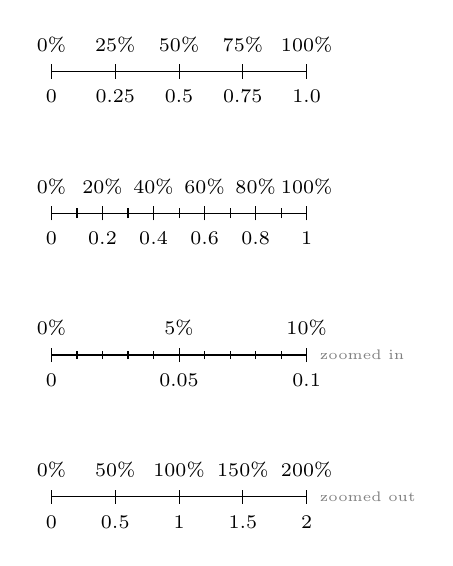
\begin{tikzpicture}[scale=0.9, every node/.style={font=\scriptsize}]

% ── Shared style ──────────────────────────────────────────────
% Each number line: width W, drawn at height Y
% Anchors labelled both sides; target marked with red ? above

% ── LINE 1: 0 to 1 in quarters (scaffolds Q5, Q7, Q3, Q4) ───
\def\Y{0}
\def\W{3.6}
\draw (0,\Y) -- (\W,\Y);
\foreach \frac/\dec/\pct in {%
    0/{0}/{0\%}, 1/{0.25}/{25\%}, 2/{0.5}/{50\%},
    3/{0.75}/{75\%}, 4/{1.0}/{100\%}}{
  \pgfmathsetmacro\xx{\frac*\W/4}
  \draw (\xx,\Y-0.10) -- (\xx,\Y+0.10);
  \node[below] at (\xx,\Y-0.13) {\dec};
  \node[above] at (\xx,\Y+0.13) {\pct};
}
% Target: 0.3 (x = 0.3*W) — red arrow, no answer

% ── LINE 2: 0 to 1 in tenths (scaffolds Q6=0.3, Q12=0.92) ───
\def\Y{-2.0}
\draw (0,\Y) -- (\W,\Y);
\foreach \k in {0,1,...,10}{
  \pgfmathsetmacro\xx{\k*\W/10}
  \pgfmathsetmacro\dec{\k/10}
  \ifodd\k
    \draw (\xx,\Y-0.07) -- (\xx,\Y+0.07); % minor tick
  \else
    \draw (\xx,\Y-0.10) -- (\xx,\Y+0.10);
    \node[below] at (\xx,\Y-0.13) {\pgfmathprintnumber[fixed,precision=1]{\dec}};
    \pgfmathsetmacro\pct{int(\k*10)}
    \node[above] at (\xx,\Y+0.13) {\pct\%};
  \fi
}
% Target: 0.92 — red marker, no answer label
\pgfmathsetmacro\ta{0.92*\W}

% ── LINE 3: 0 to 0.1 zoom (scaffolds Q8=0.08, Q11=0.005) ────
\def\Y{-4.0}
\draw (0,\Y) -- (\W,\Y);
% Anchor ticks at 0, 0.05, 0.1
\foreach \k/\dec/\pct in {0/{0}/{0\%}, 1/{0.05}/{5\%}, 2/{0.1}/{10\%}}{
  \pgfmathsetmacro\xx{\k*\W/2}
  \draw (\xx,\Y-0.10) -- (\xx,\Y+0.10);
  \node[below] at (\xx,\Y-0.13) {\dec};
  \node[above] at (\xx,\Y+0.13) {\pct};
}
% Minor ticks every 0.01
\foreach \k in {1,2,...,9}{
  \pgfmathsetmacro\xx{\k*\W/10}
  \draw (\xx,\Y-0.06) -- (\xx,\Y+0.06);
}
% Target: 0.08
% Zoom label
\node[right,gray] at (\W+0.05,\Y) {\tiny zoomed in};

% ── LINE 4: 0 to 2 (scaffolds Q10=1.4, shows >100%) ─────────
\def\Y{-6.0}
\draw (0,\Y) -- (\W,\Y);
\foreach \k in {0,1,2,3,4}{
  \pgfmathsetmacro\xx{\k*\W/4}
  \pgfmathsetmacro\dec{\k/2}
  \pgfmathsetmacro\pct{int(\k*50)}
  \draw (\xx,\Y-0.10) -- (\xx,\Y+0.10);
  \node[below] at (\xx,\Y-0.13) {\pgfmathprintnumber[fixed,precision=1]{\dec}};
  \node[above] at (\xx,\Y+0.13) {\pct\%};
}

\node[right,gray] at (\W+0.05,\Y) {\tiny zoomed out};

\end{tikzpicture}
\end{center}

\column{0.60\textwidth}
\begin{enumerate}
\begin{multicols}{2}
  \item $0.6 + 0.4 = \ablank{1}$
  \item $0.25 \times 4 = \ablank{1}$
\end{multicols}
  \item Write $\frac{3}{10}$ as a decimal: \ablank{$0.3$}
  \item Write $\frac{7}{100}$ as a decimal: \ablank{$0.07$}
\begin{multicols}{2}
  \item $0.5   = \ablank{50\%}$
  \item $0.3   = \ablank{30\%}$
  \item $0.75  = \ablank{75\%}$
  \item $0.08  = \ablank{8\%}$
  \item $0.125 = \ablank{12.5\%}$
  \item $1.4   = \ablank{140\%}$
  \item $0.005 = \ablank{0.5\%}$
  \item $0.92  \to \ablank{92\%}$
\end{multicols}
  \item \textit{Challenge:} Convert $0.0625$ to a \%,\\
        then write as a fraction in simplest form.
        \ashow{$6.25\%=\tfrac{1}{16}$}
\end{enumerate}
\end{columns}
\end{frame}

% %------------------------------------------------------------------
% % SLIDE 8: All Three Forms (unchanged)
% %------------------------------------------------------------------
% \begin{frame}[t]{Starter 8: Fractions, Decimals and Percentages}
% \vspace{-2em}
% \begin{columns}

% \column{0.38\textwidth}
% \begin{center}
% \begin{tikzpicture}[scale=0.82]
% % Conversion triangle
% \coordinate (F) at (0,0);
% \coordinate (D) at (3.2,0);
% \coordinate (P) at (1.6,2.4);
% \draw[->,thick,shorten >=4pt,shorten <=4pt] (F) -- node[below,font=\tiny]{$\div$ denom, convert} (D);
% \draw[->,thick,shorten >=4pt,shorten <=4pt] (D) -- node[right,font=\tiny]{$\times100$} (P);
% \draw[->,thick,shorten >=4pt,shorten <=4pt] (P) -- node[left,font=\tiny]{$\div100$} (F);
% \node[below left,font=\small] at (F) {\textbf{Fraction}};
% \node[below right,font=\small] at (D) {\textbf{Decimal}};
% \node[above,font=\small] at (P) {\textbf{\%}};
% % Conversion table
% \node at (1.6,-2.05) {\small
% \begin{tabular}{c|c|c}
% Fraction & Decimal & \% \\ \hline
% $\tfrac{1}{2}$ & $0.5$ & $50\%$ \\[2pt]
% $\tfrac{1}{4}$ & \ablank{0.25} & \ablank{25\%} \\[2pt]
% \ablank{$\tfrac{3}{5}$} & $0.6$ & \ablank{60\%} \\[2pt]
% \ablank{$\tfrac{7}{20}$} & \ablank{0.35} & $35\%$ \\[2pt]
% $\tfrac{1}{3}$ & \ablank{$0.\overline{3}$} & \ablank{$33.\overline{3}\%$}
% \end{tabular}};
% \end{tikzpicture}
% \end{center}

% \column{0.62\textwidth}
% \small
% \begin{multicols}{2}
% \begin{enumerate}
%   \item $0.45=\ablank{45}\%$
%   \item $72\%$ as decimal: \ablank{0.72}
%   \item $\dfrac{9}{20}$ as \%: \ablank{45\%}
%   \item $0.375$ as fraction: \ablank{$\tfrac{3}{8}$}
%   \item Order smallest to largest:\\
%         $0.6,\ \tfrac{5}{9},\ 58\%$\\
%         \ashow{$\tfrac{5}{9}{\approx}55.6\%{<}58\%{<}60\%$}

%   \columnbreak

%   \item $130\%$ as decimal: \ablank{1.3}
%   \item $1.05$ as \%: \ablank{105\%}
%   \item Which is largest?
%         \vspace{-4pt}
%         \[ \tfrac{7}{12},\quad 0.59,\quad 57\% \]
%         \vspace{-10pt}
%         \ashow{$\tfrac{7}{12}{\approx}58.3\%$ largest}
%   \item \textit{Challenge:} Order\\
%         $\tfrac{7}{9},\ 0.7\overline{8},\ 78.5\%$\\
%         \ashow{$\approx77.8\%{<}78.5\%{<}78.9\%$}
% \end{enumerate}
% \end{multicols}
% \end{columns}
% \end{frame}

% %------------------------------------------------------------------
% % SLIDE 9: Review Mix (unchanged)
% %------------------------------------------------------------------
% \begin{frame}[t]{Starter 9: Review}
% \vspace{-2.5em}
% \begin{columns}

% \column{0.28\textwidth}
% \begin{center}
% \begin{tikzpicture}[scale=0.85]
% % 0.7 bar
% \draw (0,0) rectangle (3,0.65);
% \fill[teal!35] (0,0) rectangle (2.1,0.65);
% \foreach \x in {0.3,0.6,...,2.9} \draw[gray!60] (\x,0) -- (\x,0.65);
% \node[left,font=\small] at (-0.1,0.325) {$0.7$};
% \node[right,font=\small] at (3.1,0.325) {$=\ablank{70\%}$};
% % 3/8 bar
% \draw (0,-1.1) rectangle (3,-0.45);
% \fill[purple!35] (0,-1.1) rectangle (1.125,-0.45);
% \foreach \x in {0.375,0.75,1.125,1.5,1.875,2.25,2.625}
%   \draw (\x,-1.1) -- (\x,-0.45);
% \node[left,font=\small] at (-0.1,-0.775) {$\tfrac{3}{8}$};
% \node[right,font=\small] at (3.1,-0.775) {$=\ablank{37.5\%}$};
% % Number line 0–100%
% \draw (-0.1,-2.1) -- (3.1,-2.1);
% \foreach \x/\lab in {0/{$0\%$},1.5/{$50\%$},3/{$100\%$}}{
%   \draw (\x,-2.2) -- (\x,-2.0);
%   \node[below,font=\tiny] at (\x,-2.28) {\lab};
% }
% \draw[red,thick] (1.125,-2.25) -- (1.125,-1.95);
% \draw[blue,thick] (2.1,-2.25) -- (2.1,-1.95);
% \end{tikzpicture}
% \end{center}

% \column{0.72\textwidth}
% \small
% \begin{multicols}{2}
% \begin{enumerate}
%   \item $\dfrac{3}{4}=\ablank{75}\%$
%   \item $0.06=\ablank{6}\%$
%   \item $\dfrac{5}{8}=\ablank{62.5}\%$
%   \item $110\%$ as decimal: \ablank{1.1}
%   \item $35\%$ of \pounds60 $={}$\pounds\ablank{21}
%   \item Increase \pounds80 by $15\%$: \ablank{\pounds92}

%   \columnbreak

%   \item Decrease 240 by $12.5\%$: \ablank{210}
%   \item $\dfrac{2}{3}+15\%={}$\ablank{$81.\overline{6}\%$}
%   \item Order: $0.7,\ \tfrac{3}{4},\ 72\%$\\
%         \ashow{$70\%<72\%<75\%$}
%   \item \textit{Challenge:} Item: $-20\%$, then $-10\%$ more. Same as $-30\%$?\\
%         \ashow{$\times0.8\times0.9{=}\times0.72$. That's $28\%$ off, not $30\%$!}
% \end{enumerate}
% \end{multicols}
% \end{columns}
% \end{frame}

\end{document}